\section{Descrizione architettura}
% Nell'indice proposto da Tullio c'è:
% a. Metodo e formalismo di specifica
% b. Presentazione dell'architettura generale del sistema e identificazione dei componenti architetturali di alto livello

\subsection{Metodo e formalismo di specifica}

Le scelte progettuali per lo sviluppo di \ProjectName{} sono state fortemente influenzate dallo stack tecnologico utilizzato.

In primo luogo il progetto è basato su Node.js ed è scritto quindi in JavaScript: un linguaggio che è (tra le altre caratteristiche) orientato agli oggetti (\glossario{OOP}), ma che lascia grande libertà al programmatore nella scelta della tecnica da utilizzare per l'implementazione di pattern come l'\glossario{incapsulamento} e l'\glossario{ereditarietà}. Al contrario di altri linguaggi (C++, Java) non c'è un costrutto esplicito con il quale il programmatore può definire classi. 

Progettare il sistema con un'architettura ad oggetti classica non permette di rappresentare in modo immediato la gestione dinamica dei tipi e le caratteristiche tipiche degli stili di programmazione funzionali. In certi casi è stato necessario introdurre interfacce ``fittizie'', che non verranno codificate. Dato che questo introduce numerosi schematismi che appesantiscono i diagrammi e che non sono richiesti dal linguaggio di programmazione, si è cercato di limitarli soltanto ai casi in cui sono particolarmente utili.

Il nostro approccio alla progettazione è stato contemporaneamente top-down e bottom-up. Da un lato siamo partiti suddividendo il sistema in front-end e back-end, definendo l'interfaccia di comunicazione, scegliendo di seguire in ciascuno l'organizzazione suggeritaci dai framework (Express e AngularJS). Dall'altro lato siamo partiti dal basso, componendo e cercando di riutilizzare il più possibile le librerie già esistenti. Per far questo abbiamo prima cercato e confrontato con attenzione la struttura e le scelte sia di progetti open-source che di progetti proposti come best-practise.

L'approccio top-down è stato schematizzato nei diagrammi di deployment e dei package. Per la costruzione dei diagrammi delle classi, invece, questo approccio si è rivelato essere molto poco produttivo e rigoroso. I diagrammi delle classi proposti sono quindi \emph{uno dei possibili diagrammi} che descrivono l'applicazione, qualsiasi gerarchia o relazione complicata tra le classi verrebbe tradotta pressapoco nello stesso codice.

Per descrivere il sistema si è rivelato molto più comodo utilizzare i diagrammi di sequenza e di attività in un approccio bottom-up, descrivendo l'interazione tra i singoli oggetti senza preoccuparci della loro classificazione. In questo modo siamo anche riusciti a descrivere alcuni dei meccanismi tipici dell'applicazione, in particolar modo l'ordine in cui agiscono i \glossario{middleware} di Express. Riteniamo che saranno molto utili per la progettazione di dettaglio e per la codifica.

I diagrammi di deployment, dei \glossario{package}, delle classi, di sequenza e di attività presentati di seguito utilizzano la specifica \glossario{UML} 2.0.

\subsection{Diagramma di deployment e REST}
%TODO Diagramma di deployment client server al posto dello schema colorato
\glossario{REST}, ovvero \textit{Representational State Transfer} è un tipo di \glossario{RPC}. Si basa su un protocollo di comunicazione \glossario{stateless} di tipo client-server (solitamente \glossario{HTTP} ed è stato scelto anche per \ProjectName{}.

I motivi che hanno spinto alla scelta di \glossario{REST} sono:
\begin{itemize}
\item Semplicità di utilizzo;
\item Indipendenza dal sistema operativo utilizzato dal client;
\item Indipendenza dai linguaggi di programmazione utilizzati;
%\item In coppia con HTTPS permette una certa sicurezza delle comunicazioni.
\end{itemize}

\glossario{REST} utilizza il concetto di risorsa, ovvero un aggregato di dati con un nome (\glossario{URI}) e una rappresentazione, su cui è possibile invocare le operazioni \glossario{CRUD} tramite il protocollo sopracitato.

Nell'\glossario{URI} inviato sono presenti il nome della risorsa e la sua rappresentazione, identificata dall'estensione del file scelto, e per \ProjectName{} è stato scelto il formato \glossario{JSON}, in quanto il suo \glossario{parsing} in \glossario{JavaScript} è più semplice rispetto, ad esempio, a quello di \glossario{XML} o \glossario{CSV}.

Un'altra caratteristica di \glossario{REST} è che essendo \glossario{stateless} ogni richiesta dovrà contenere tutte le informazioni necessarie in modo indipendente dallo stato del sistema.

\subsection{Architettura generale}

L'architettura scelta per lo sviluppo di \ProjectName{} si serve del \glossario{design pattern} \glossario{MVC} (\textit{Model-View-Controller}). Nel diagramma in figura \ref{architetturaGeneralePackage} viene presentata la struttura ad alto livello, evidenziando le componenti che ricoprono i ruoli di \textit{model} e \textit{controller} per il \glossario{back-end}, e controller per il \glossario{front-end}. Il \glossario{back-end} non presenta la \textit{view} poiché, utilizzando il formato \glossario{JSON}, la conversione dalla rappresentazione interna alla presentazione testuale (\glossario{JSON}) è automatica e diretta.
Il \glossario{front-end} è gestito dal \glossario{framework} \glossario{AngularJS}, la cui architettura è stata per diversi anni vicina al modello \glossario{MVC}. Nel tempo si è avvicinato più al modello \glossario{MVVM}. Ora \glossario{AngularJS} si dichiara \glossario{MVW} ossia Model-View-Whatever\footnote{Si rimanda al sito ufficiale di AngularJS: \url{http://angularjs.org/}}, per la caratteristica di non corrispondere esattamente ad uno dei modelli classici. Nell'architettura scelta per \ProjectName{}, si è scelto di descrivere soltanto i \glossario{package} che compongono il controller, perché l'aggiornamento della view e del model viene gestito da \glossario{AngularJS} internamente.

\begin{figure}[H] %TODO modificare
\centering
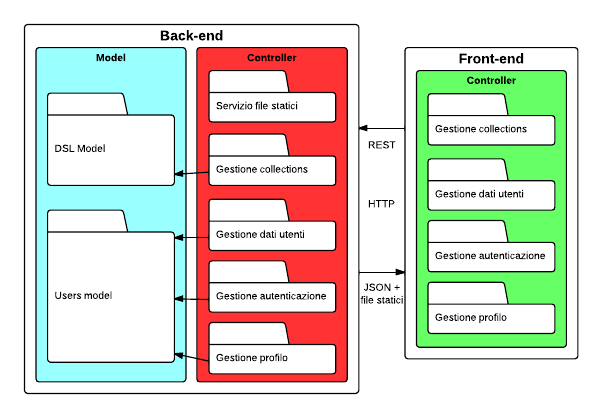
\includegraphics[width=\textwidth]{uml/architettura-generale-package.png}
\caption{Architettura generale dei package}
\label{architetturaGeneralePackage}
\end{figure}

\subsubsection{Back-end}
\subsubsection{Front-End}